\section{Methodology}\label{sec:method}

\begin{figure*}[!tphb]
    \centering
    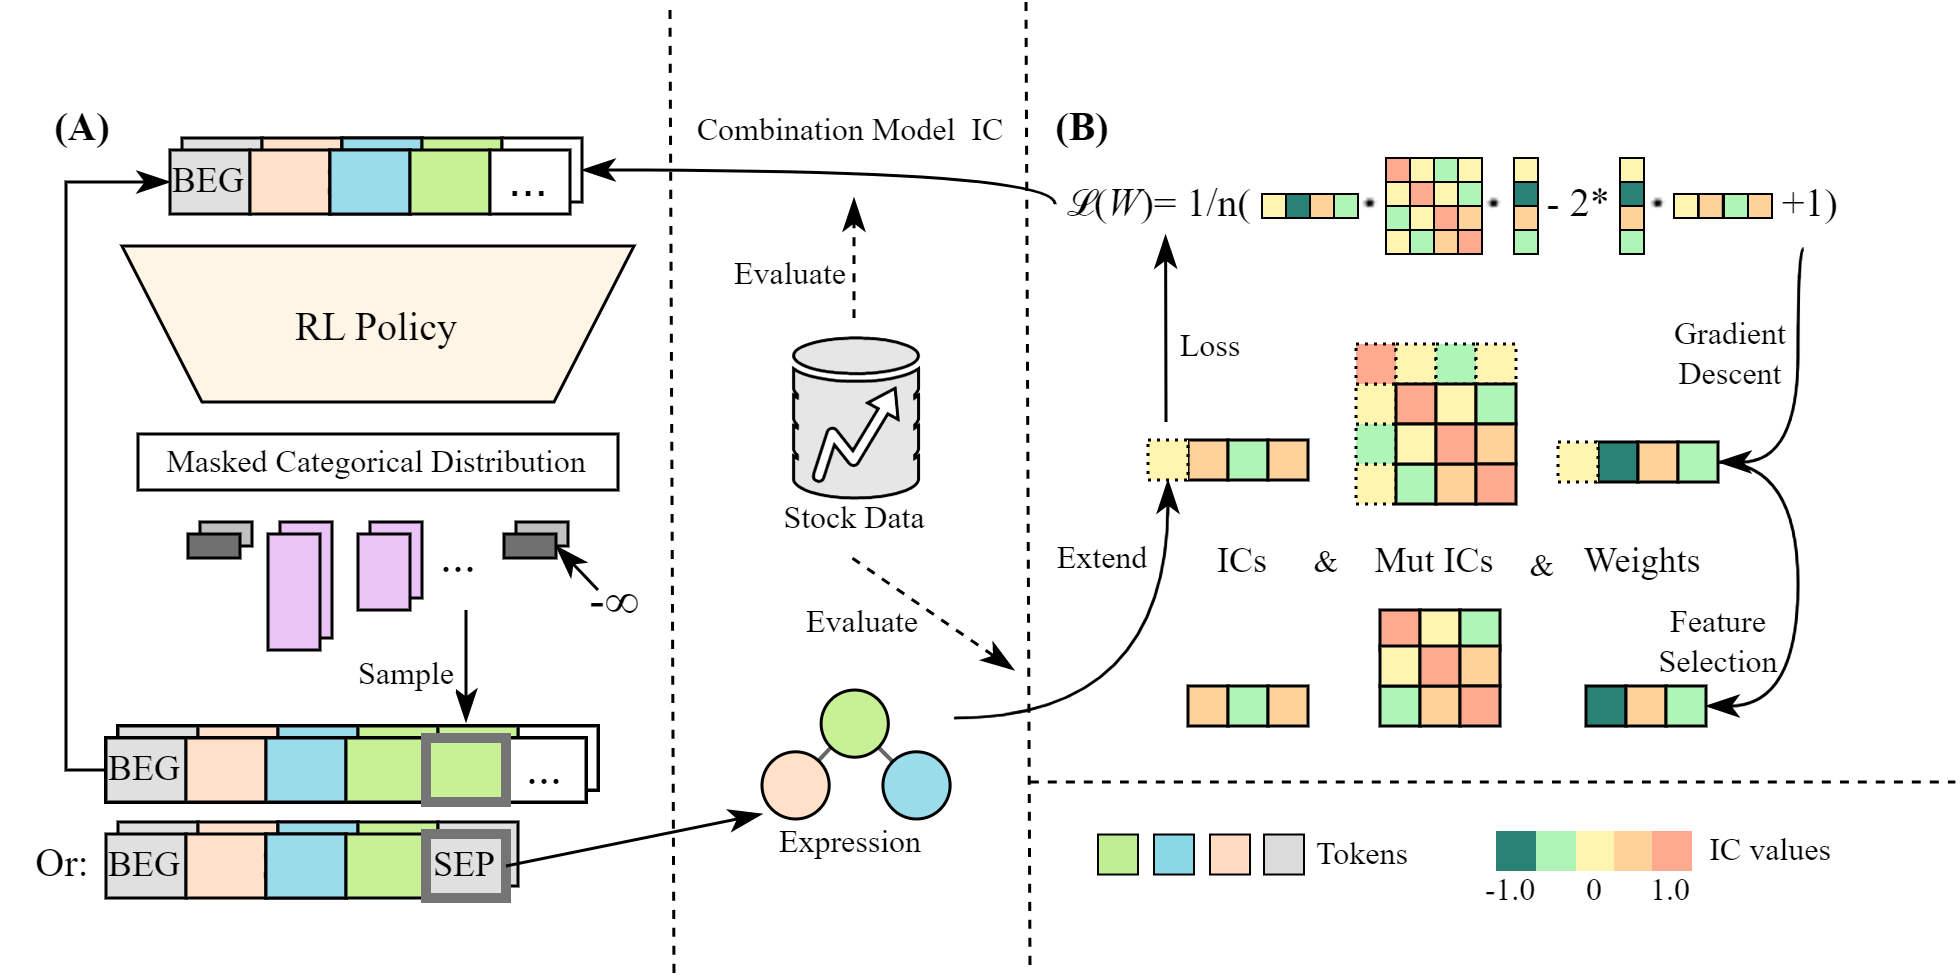
\includegraphics[width=0.8\linewidth]{Images/main.png}
    \caption{An overview of our alpha-mining framework. (A) An alpha generator that generates expressions, optimized via a policy gradient algorithm. (B) A combination model that maintains a weighted combination of principal factors and, in the meantime, provides evaluative signals to guide the generator.}
    \Description{}
    \label{fig:main}
\end{figure*}


As illustrated in Figure \ref{fig:main}, our alpha-mining framework consists of two main components: 1) the \emph{Alpha Combination Model}, which combines multiple formulaic alphas to achieve optimal performance in prediction, and 2) the \emph{RL-based Alpha Generator}, which generates formulaic alphas in the form of a token sequence. The performance of the Alpha Combination Model is used as the reward signal to train the RL policy in the Alpha Generator using policy gradient-based algorithms, such as PPO \cite{ppo}. Repeating this process, the generator is continuously trained to generate alphas that boost the combination model, thereby enhancing the overall predictive power.

\subsection{Alpha Combination Model}  \label{sec:alpha_improvement}

Considering the interpretability of the combined ``mega-alpha'', the combination model itself should also be interpretable. In this paper, we use a linear model to combine the alphas.

The values evaluated from different alphas have drastically different scales, which might cause problems in the following optimization steps. To counter this effect, we centralize and normalize the alpha values with their average and standard deviation. Since Pearson's correlation coefficient is invariant up to linear transformation, this transformation does not affect the performance of the alphas when they are considered separately. Formally, we introduce a normalization operator $\mathcal{N}$, that transforms a vector such that its elements have a mean of 0, and the vector has a length of 1:
\begin{equation}
    \brackets{\mathcal{N}(u)}_i = \frac{u_i - \bar{u}}
    {\sqrt{\sum_{j=1}^n\parens{u_j - \bar{u}}^2}}.
\end{equation}

We will omit explicitly writing the $\mathcal{N}$ operator for simplicity. For the rest of this paper, we will assume that all the $f(X)$ evaluations and the targets $y$ are normalized to have a mean of 0 and a length of 1 before subsequent computations. In other words, treat $f$ as $\mathcal{N} \circ f$ and $y$ as $\mathcal{N}(y)$.

Given a set of $k$ alpha factors $\mathcal{F} = \braces{f_1, f_2, \cdots, f_k}$ and their weights $w = \parens{w_1, w_2, \cdots, w_k} \in \mathbb{R}^k$, the combination model $c$ is defined as follows:
\begin{equation}
    c(X; \mathcal{F}, w)
    = \sum_{j=1}^{k} w_j f_j(X) = z.
\end{equation}

We define the loss of the combination model as the mean squared error (MSE) between model outputs and true stock trend values:
\begin{equation}
    \mathcal{L}(w) = \frac{1}{nT}\sum_{t=1}^{T} \|z_t - y_t\|^2.
\end{equation}

To simplify the calculation of alpha combination, we have:

\begin{theorem} \label{thm:loss_transformation}
Let $\mathcal{F}$ be a set of $k$ alphas and $w$ be their respective weights, the MSE loss $\mathcal{L}(w)$ can be represented as:

\begin{equation} \label{eq:model_loss}
    \begin{aligned}
        \mathcal{L}(w) = \frac{1}{n} \parens{
            1 - 2 \sum_{i=1}^{k} w_i \bar{\sigma}_y(f_i) + \sum_{i=1}^{k} \sum_{j=1}^{k} w_i w_j \bar{\sigma}(f_i(X), f_j(X))
        }.
    \end{aligned}
\end{equation}

\end{theorem}

The proof of this theorem is provided in Appendix \ref{sec:thm_proof}. Notice that there is no $z_t$ term on the RHS of Equation \ref{eq:model_loss}. Once we have obtained $\bar{\sigma}_{y}(f)$ for each alpha $f$ and their pairwise mutual correlations $\bar{\sigma}(f_i(X),f_j(X))$, we can then calculate the loss $\mathcal{L}(w)$ solely using these terms, saving time on calculating the relatively large $z_t$ in each gradient descent step.
 
Considering time and space complexity, it is impractical to combine all generated alphas together, because to calculate mutual correlation for each pair of factors we need $\mathcal{O}(k^2)$ evaluations of mutual IC. The quadratic growth of this makes it expensive to apply the current procedure to a large number of alphas. However, a few dozen of alphas will suffice for practical uses. To a certain point, more alphas would not bring much more increment in performance, following the law of diminishing returns. We will demonstrate this effect in Section \ref{sec:ablation}.

\begin{algorithm}
\caption{Incremental Combination Model Optimization}
\label{alg:model}
\KwInput {Alpha set $\mathcal{F} = \braces{f_1, \cdots, f_k}$, weights $w = \braces{w_1, \cdots, w_k}$ and a new alpha $f_\textrm{new}$}
\KwOutput {Optimal alpha subset $\mathcal{F}^* = \braces{f_1', \cdots, f_k'}$, optimal weights $w^* = \parens{w_1', \cdots, w_k'}$}
$\mathcal{F}\gets \mathcal{F}\cup \braces{f_\textrm{new}}, w\gets w \Vert \mathrm{rand}()$;\\
\ForEach{$f \in \mathcal{F}$}{
    Obtain $\bar{\sigma}_y(f)$ from calculation or cache;\\
    \ForEach{$f' \in \mathcal{F}$}{
        Obtain $\bar{\sigma}(f(X), f'(X))$ from calculation or cache;
    }
}
\For{$i\gets1$ \KwTo $num\_gradient\_steps$}{
    Calculate $\mathcal{L}(w)$ according to Equation \ref{eq:model_loss};
    $w \gets \mathrm{GradientDescent}(\mathcal{L}(w))$;
}
$p \gets \argmin_i |w_i|$;\\
$\mathcal{F} \gets \mathcal{F}\backslash \braces{f_p}$, $w \gets \parens{w_1, \cdots, w_{p-1}, w_{p+1}, \cdots, w_k}$;\\
\Return $\mathcal{F}, w$;
\end{algorithm}

After the alpha generator outputs a new alpha, the alpha is first added to the candidate alpha set and assigned a random initial weight. Gradient descent is then performed to optimize the weights with respect to the extended alpha set. We also set a threshold to limit the size of the alpha set, leaving only the principal alphas with the largest absolute weight. If the amount of alphas in the extended set exceeds a certain threshold, the least principal alpha is removed from the set together with its corresponding weight. The pseudocode of the training procedure is shown in Algorithm \ref{alg:model}.
